\documentclass{tudelft-report}

%% Set up section numbering without chapters
\counterwithout{section}{chapter}

%% Set up the bibliography
\usepackage{biblatex}
\addbibresource{report.bib}

%% Additional packages and commands
\usepackage{parskip}
\setlist{itemsep=-2pt} % Reducing white space in lists slightly
\renewcommand{\deg}{\si{\degree}\xspace} % Use \deg easily, everywhere

%% ----------------------------------------------------------------------
%%    Begin of document
%% ----------------------------------------------------------------------

\begin{document}

%% Define main cover parameters
\title{Reinforcement Learning for Lander Control}
%\subtitle{AE4350 Technical Report}
\author{Andreu Craus Vidal (6552501)}

\subject{AE4350: Bio-inspired Intelligence and Learning for Aerospace Applications} % Cover only
\affiliation{Delft University of Technology} % Cover only
\coverimage{figures/Cover_Gemini_3.jpg} % Aspect ratio of 2:3 (portrait) recommended
\definecolor{title}{HTML}{4884d6} % Color for cover title

\makecover
\pagenumbering{arabic}

\begin{titlepage}

\begin{center}

%% Print the title
{\makeatletter
\largetitlestyle\fontsize{40}{40}\selectfont\@title
\makeatother}

%% Print the subtitle
{\makeatletter
\ifdefvoid{\@subtitle}{}{\bigskip\titlestyle\fontsize{18}{18}\selectfont\@subtitle}
\makeatother}

\bigskip
\bigskip

by

\bigskip
\bigskip

%% Print the name of the author
{\makeatletter
\largetitlestyle\fontsize{22}{22}\selectfont\@author
\makeatother}

\bigskip
\bigskip

%% Print table with student details and repository
\setlength\extrarowheight{3pt}
\begin{tabular}{ll}
    \textbf{Student Name:} & Andreu Craus Vidal \\
    \textbf{Student Number:} & 6552501 \\
    \textbf{GitHub Repository:} & \url{https://github.com/acrausvidal/BioInspired_2026_lander_project} \\
\end{tabular}

\vfill

%% Print course and faculty information
\begin{tabular}{ll}
    \textbf{Course:} & AE4350 Bio-inspired Intelligence and Learning for Aerospace Applications \\
    \textbf{Instructors:} & Guido de Croon, Erik-Jan van Kampen \\
    \textbf{Project Duration:} & 2025-2026 Q4 \\
    \textbf{Faculty:} & Faculty of Aerospace Engineering, Delft University of Technology \\
\end{tabular}

\bigskip
\bigskip

%% Add a source and description for the cover and optional attribution for the template
\begin{tabular}{p{15mm}p{10cm}}
    Cover: & Artwork by Nanobanana \\
    Style: & TU Delft Report Style, with modifications by Daan Zwaneveld
\end{tabular}

\end{center}

%% Insert the TU Delft logo at the bottom of the page
\begin{tikzpicture}[remember picture, overlay]
    \node[above=10mm] at (current page.south) {%
        
\includegraphics{figures/logo-black}
    };
\end{tikzpicture}

\end{titlepage}


\tableofcontents

\newpage
\section*{Abbreviations}

\begin{longtable}{p{2.5cm}p{10cm}}
    \toprule
    Abbreviation & Definition                       \\
    \midrule\endhead
    AC           & Actor-Critic                     \\
    ACD          & Adaptive Critic Design           \\
    ANN          & Artificial Neural Network        \\
    GAE          & Generalized Advantage Estimation \\
    MLP          & Multi-Layer Perceptron           \\
    MSE          & Mean Squared Error               \\
    PPO          & Proximal Policy Optimization     \\
    RCS          & Reaction Control System          \\
    RL           & Reinforcement Learning           \\
    TD           & Temporal Difference              \\
    \bottomrule
\end{longtable}

\section*{Symbols}

\begin{longtable}{p{2.5cm}p{9.5cm}p{2.0cm}}
    \toprule
    Symbol                   & Definition                                         & Unit                         \\
    \midrule\endhead
    $\hat{A}_t$              & Advantage function estimate                        & [-]                          \\
    $c_{\text{ent}}$         & Policy entropy bonus coefficient                   & [-]                          \\
    $c_v$                    & Value loss weighting coefficient                   & [-]                          \\
    $F(t)$                   & Instantaneous fuel capacity / remaining fuel       & [units]                      \\
    $F_0$                    & Initial total fuel capacity ($100.0$)              & [units]                      \\
    $g$                      & Gravitational acceleration ($10.0$)                & [$\text{m/s}^2$]             \\
    $I_{zz}(t)$              & Mass moment of inertia about pitch axis            & [$\text{kg}\cdot\text{m}^2$] \\
    $m(t)$                   & Total lander mass                                  & [kg]                         \\
    $r_t$                    & Scalar reward at time step $t$                     & [-]                          \\
    $R_t$                    & Discounted cumulative return                       & [-]                          \\
    $s_t$                    & Environment state observation vector               & [-]                          \\
    $t$                      & Discrete simulation time step                      & [s]                          \\
    $u_t$                    & Continuous action vector $[u_1, u_2]$              & [-]                          \\
    $u_{\text{main}}$        & Main engine throttle ($[0.5, 1.0]$)                & [-]                          \\
    $u_{\text{side}}$        & Lateral thruster throttle ($[-1.0, 1.0]$)          & [-]                          \\
    $v_x, v_y$               & Horizontal and vertical linear velocities          & [m/s]                        \\
    $V(s)$                   & State-value function                               & [-]                          \\
    $x, y$                   & Planar coordinates relative to landing pad         & [m]                          \\
    \midrule
    $\alpha$                 & Neural network learning rate                       & [-]                          \\
    $\gamma$                 & Future reward discount factor                      & [-]                          \\
    $\delta_t$               & Temporal Difference (TD) residual                  & [-]                          \\
    $\epsilon_{\text{clip}}$ & PPO clipping threshold ($0.20$)                    & [-]                          \\
    $\theta$                 & Pitch orientation angle                            & [rad]                        \\
    $\lambda$                & GAE exponential weighting factor ($0.95$)          & [-]                          \\
    $\mu(s)$                 & Mean of Gaussian policy action distribution        & [-]                          \\
    $\pi(u \mid s)$          & Control policy                                     & [-]                          \\
    $\rho(t)$                & Lander body density                                & [$\text{kg/m}^2$]            \\
    $\rho_0$                 & Initial wet body density ($5.0$)                   & [$\text{kg/m}^2$]            \\
    $\rho_{\text{dry}}$      & Dry body density ($2.5$)                           & [$\text{kg/m}^2$]            \\
    $\sigma$                 & Standard deviation of Gaussian policy distribution & [-]                          \\
    $\phi$                   & Critic neural network weights                      & [-]                          \\
    $\omega$                 & Pitch angular velocity                             & [rad/s]                      \\
    \bottomrule
\end{longtable}


%% ----------------------------------------------------------------------
%%    Main Report Sections (AE4350 Grading Rubric)
%% ----------------------------------------------------------------------

\newpage
\section{Introduction}
\label{sec:introduction}

\emph{An introduction to the lander reinforcement learning project...}


\section{System Description and Physical Modeling}
\label{sec:system_description}

\subsection{Coordinate Frames of Reference}
To establish an unambiguous kinematic and dynamic representation of the powered descent vehicle, two Cartesian coordinate frames are defined in accordance with standard aerospace flight mechanics conventions:
\begin{enumerate}[leftmargin=*,label=\textbf{\arabic*.}]
    \item \textbf{Inertial Landing Frame} $\mathcal{F}_I = \{O_I, \vec{x}_I, \vec{y}_I\}$: An earth/lunar-fixed frame where the origin $O_I$ is anchored at the midpoint of the designated landing helipad. The unit vector $\vec{x}_I$ extends horizontally parallel to the ground plane, and $\vec{y}_I$ extends vertically upward, collinear with the local gravity vector opposite to lunar gravitation.
    \item \textbf{Body-Fixed Frame} $\mathcal{F}_B = \{O_B, \vec{x}_B, \vec{y}_B\}$: A vehicle-fixed reference frame centered at the instantaneous center of mass $O_B$. The longitudinal axis $\vec{y}_B$ aligns with the vertical centerline of the lander fuselage along the thrust vector of the main engine, while the lateral axis $\vec{x}_B$ points toward the starboard landing gear.
\end{enumerate}

The vehicle attitude is parameterized by the planar pitch orientation angle $\theta(t) \in [-\pi, \pi]$, defined as the right-handed rotation angle between the inertial vertical $\vec{y}_I$ and the body longitudinal axis $\vec{y}_B$. An orientation of $\theta = 0$ corresponds to a nominal upright flight condition, with counter-clockwise angular displacement designated as positive.

\subsection{Planar Non-Linear Flight Dynamics}
The lunar lander is modeled as a 3-Degree-of-Freedom (3-DOF) planar rigid body subject to non-linear gravitational, thrust, aerodynamic disturbance, and contact forces. The governing continuous-time translational and rotational equations of motion expressed in the inertial frame are formulated as:
\begin{align}
    \ddot{x}(t) &= \frac{-F_{\text{main}}(t)\sin\theta(t) - F_{\text{side}}(t)\cos\theta(t) + F_{\text{wind},x}(t)}{m(t)}, \label{eq:eom_x} \\
    \ddot{y}(t) &= \frac{F_{\text{main}}(t)\cos\theta(t) - F_{\text{side}}(t)\sin\theta(t) + F_{\text{wind},y}(t)}{m(t)} - g, \label{eq:eom_y} \\
    \ddot{\theta}(t) &= \frac{M_{\text{thrust}}(t) + M_{\text{turb}}(t)}{I_{zz}(t)}, \label{eq:eom_theta}
\end{align}
where $g = 10.0\,\si{m/s^2}$ denotes the scaled gravitational acceleration constant, $m(t)$ represents the instantaneous vehicle mass, and $I_{zz}(t)$ denotes the time-varying mass moment of inertia about the out-of-plane rotation axis. The thrust terms $F_{\text{main}}$ and $F_{\text{side}}$ are modulated by the autonomous controller, while $F_{\text{wind}}$ and $M_{\text{turb}}$ simulate stochastic aerodynamic disturbances parameterized through non-linear sinusoidal and tanh functions \cite{towers2023gymnasium}.

\subsection{Dynamic Mass Variation and Fuel Depletion Model}
Unlike standard benchmark environments that assume constant vehicle mass, realistic rocket-powered descent trajectories are governed by Tsiolkovsky mass depletion dynamics. As propellant is expelled through continuous throttle firings, the physical mass of the lander body continuously declines from its initial fully-fueled ("wet") condition to its empty ("dry") structural state.

The vehicle is initialized with a total propellant capacity of $F_0 = 100.0\,\text{units}$. The instantaneous propellant volume $F(t)$ is governed by the mass flow rate differential equation:
\begin{equation}
    \dot{F}(t) = - \left( u_{\text{main}}(t) \cdot \dot{m}_{\text{main,max}} + |u_{\text{side}}(t)| \cdot \dot{m}_{\text{side,max}} \right), \quad F(0) = F_0,
    \label{eq:fuel_depletion}
\end{equation}
where $\dot{m}_{\text{main,max}} = 0.40\,\text{units/step}$ ($20.0\,\text{units/s}$ at $50\,\si{Hz}$) and $\dot{m}_{\text{side,max}} = 0.05\,\text{units/step}$ ($2.5\,\text{units/s}$ at $50\,\si{Hz}$) represent the maximum mass consumption rates for the main engine and reaction control system (RCS) thrusters, respectively. 

To simulate continuous mass and inertia tensor recalculation within the Box2D multi-body physics engine, the structural polygon density $\rho(t)$ is dynamically coupled to the normalized remaining fuel fraction $f(t) = F(t)/F_0 \in [0.0, 1.0]$:
\begin{equation}
    \rho(t) = \rho_{\text{dry}} + (\rho_0 - \rho_{\text{dry}}) \cdot f(t),
    \label{eq:density_scaling}
\end{equation}
with wet density $\rho_0 = 5.0\,\si{kg/m^2}$ (total wet mass $m_{\text{wet}} \approx 4.82\,\si{kg}$) and dry density $\rho_{\text{dry}} = 2.5\,\si{kg/m^2}$ (dry mass $m_{\text{dry}} \approx 2.41\,\si{kg}$). At every discrete integration step $\Delta t = 1/50\,\si{s}$, the density of the polygonal body fixtures is refreshed and the rigid body inertia tensor is updated via \texttt{body.ResetMassData()}. Consequently, as propellant depletes, the control authority $\vec{F}/m(t)$ increases dynamically by a factor of $2.0$, requiring the learning agent to synthesize an adaptive policy robust to shifting plant transfer functions.

\subsection{Actuator Mechanics and Landing Gear Multi-Body Constraints}
The control interface operates over a 2-dimensional continuous vector $\mathbf{u} = [a_1, a_2]^T \in [-1.0, 1.0]^2$. The continuous actuator commands map non-linearly to physical engine throttles:
\begin{itemize}[leftmargin=*,label=$\bullet$]
    \item \textbf{Main Engine ($a_1$):} Generates pure axial thrust along the positive $\vec{y}_B$ vector. To reflect realistic rocket engine minimum ignition thresholds, a non-linear activation envelope is enforced:
    \begin{equation}
        u_{\text{main}} = \begin{cases}
            0, & \text{if } a_1 \le 0, \\
            0.5 \cdot (a_1 + 1.0) \in [0.5, 1.0], & \text{if } a_1 > 0.
        \end{cases}
        \label{eq:main_actuator}
    \end{equation}
    The resulting thrust magnitude is $F_{\text{main}}(t) = u_{\text{main}}(t) \cdot T_{\text{main,max}}$, where $T_{\text{main,max}} = 13.0\,\si{N}$.
    \item \textbf{Lateral Thrusters ($a_2$):} Provide directional differential torque for attitude stabilization and horizontal translation. A deadband region is established to avoid continuous jitter:
    \begin{equation}
        u_{\text{side}} = \begin{cases}
            0, & \text{if } |a_2| \le 0.5, \\
            \text{sign}(a_2) \cdot |a_2| \in [-1.0, -0.5] \cup [0.5, 1.0], & \text{if } |a_2| > 0.5.
        \end{cases}
        \label{eq:side_actuator}
    \end{equation}
    The RCS thruster provides a force of $F_{\text{side}}(t) = |u_{\text{side}}(t)| \cdot T_{\text{side,max}}$ with $T_{\text{side,max}} = 0.6\,\si{N}$, located at moment arms $h_{\text{side}} = 14/30\,\si{m}$ and $d_{\text{side}} = 12/30\,\si{m}$ relative to the vehicle center of mass.
\end{itemize}

The landing gear assembly consists of two articulated cantilever legs connected via revolute joints to the fuselage. Each joint incorporates an active linear torsional spring ($\tau_{\text{spring}} = 40\,\si{N\cdot m}$) and angular mechanical limiters ($[-0.4, 0.9]\,\si{rad}$ starboard, $[-0.9, 0.4]\,\si{rad}$ port) to absorb touchdown impact energy. A high-frequency contact detector monitors ground collisions.

\subsection{Operational Envelope and Terminal Conditions}
An episode terminates upon encountering one of three mutually exclusive operational boundary conditions:
\begin{enumerate}[leftmargin=*,label=\textbf{\arabic*.}]
    \item \textbf{Safe Touchdown (Success):} The lander comes to complete rest ($\|\mathbf{v}\| \le 0.05\,\si{m/s}$, $\omega \le 0.05\,\si{rad/s}$), the body orientation is upright ($|\theta| \le 0.1\,\si{rad}$), and both landing leg sensors maintain stable ground contact within the helipad boundary ($r_{\text{term}} = +100.0$).
    \item \textbf{Catastrophic Crash (Failure):} The central fuselage contacts the terrain, the vehicle overturns ($|\theta| \ge \pi/2$), or the vehicle drifts beyond horizontal limits $|x| \ge 1.0$ ($r_{\text{term}} = -100.0$).
    \item \textbf{Fuel Exhaustion (Failure):} Propellant drops to zero ($F(t) \le 0$) prior to securing a safe surface state, extinguishing all engine thrust and incurring an immediate catastrophic penalty ($r_{\text{term}} = -100.0$).
\end{enumerate}

\newpage
\section{Continuous RL Controller Design}
\label{sec:rl_controller_design}

\subsection{Reinforcement Learning Framework}
In Reinforcement Learning, the flight controller acts as an \emph{agent} interacting with the simulated flight environment through a continuous feedback loop \cite{vankampen2025lecture, sutton2018reinforcement}. At each time step $t$, the agent receives a state observation $s_t$ from the environment, selects a continuous control action $u_t$, and receives a scalar reward $r_t$ alongside the next state $s_{t+1}$.

The goal of the agent is to learn an optimal policy $\pi(u \mid s)$ that maximizes the expected cumulative discounted future reward, known as the \emph{value function} $V(s)$ \cite{vankampen2025lecture}:
\begin{equation}
    V(s) = \mathbb{E} \left[ \sum_{k=0}^{\infty} \gamma^k r_{t+k+1} \; |\; s_t = s \right],
    \label{eq:value_function}
\end{equation}
where $\gamma \in [0, 1)$ is the discount factor specifying how much future rewards are valued relative to immediate rewards. Using the recursive Bellman property, the value function satisfies \cite{vankampen2025lecture}:
\begin{equation}
    V(s) = \mathbb{E} \left[ r_{t+1} + \gamma V(s_{t+1}) \; | \; s_t = s \right].
    \label{eq:bellman_equation}
\end{equation}

\subsection{Actor-Critic Architecture and Function Approximation}
For simple discrete tasks, value functions can be stored in lookup tables (e.g., standard Q-tables). However, discretizing a continuous 9-dimensional state space and a 2-dimensional continuous action space creates an intractable curse of dimensionality. For continuous flight control, function approximators such as Artificial Neural Networks (ANNs) are necessary \cite{vankampen2025lecture}.

In this context, an \textbf{Actor-Critic} (or Adaptive Critic Design) architecture with to distinct ANNs is utilized:
\begin{itemize}[leftmargin=*,label=$\bullet$]
    \item \textbf{Critic Network ($V_\phi$):} Approximates the value function $V(s)$. The network takes the 9-dimensional state vector as input and outputs a single scalar estimating the expected future return of that state.
    \item \textbf{Actor Network ($\pi_\theta$):} Represents the control policy mapping states directly to continuous actions. The network takes the 9-dimensional state vector and parameterizes a Gaussian distribution $\mathcal{N}(\mu(s), \sigma^2)$, outputting the mean action $\mu(s)$ and a trainable standard deviation $\sigma$ for each control channel.
\end{itemize}
Both the Actor and Critic networks are implemented as Multi-Layer Perceptrons (MLPs) with two fully connected hidden layers of 128 neurons each\footnote{This architecture aligns with standard, benchmarked configurations in prominent reinforcement learning frameworks such as those in Stable-Baselines3 \cite{raffin2021stable}. A $128\times 128$ hidden layer size is widely utilized to balance function approximation capacity with training stability and sample efficiency.} and Hyperbolic Tangent ($\tanh$) activation functions.

% \begin{figure}[H]
%     \centering
%     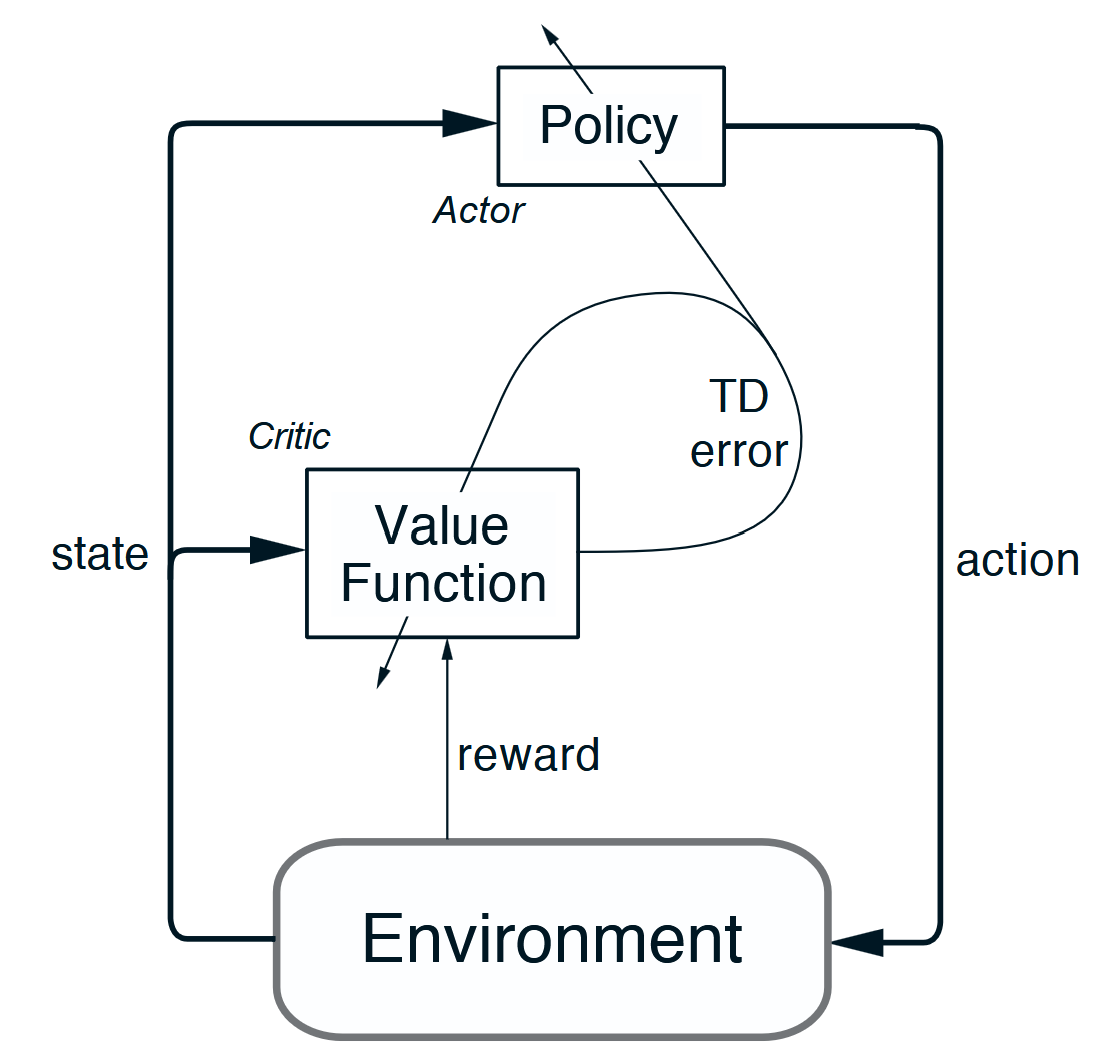
\includegraphics[width=0.45\linewidth]{figures/AC_architecture.png}
%     \caption{The actor-critic architecture \cite{sutton2018reinforcement}.}
%     \label{fig:AC_architecture}
% \end{figure}

\subsection{Proximal Policy Optimization (PPO)}
Standard actor-critic algorithms can suffer from high training instability if a gradient step causes a large, destructive policy update. Proximal Policy Optimization (PPO) \cite{schulman2017proximal} resolves this by clipping the policy probability ratio $r_t(\theta) = \frac{\pi_\theta(u_t \mid s_t)}{\pi_{\theta_{\text{old}}}(u_t \mid s_t)}$:
\begin{equation}
    L^{\text{CLIP}}(\theta) = \hat{\mathbb{E}}_t \left[ \min\left( r_t(\theta)\hat{A}_t, \, \text{clip}(r_t(\theta), 1-\epsilon_{\text{clip}}, 1+\epsilon_{\text{clip}})\hat{A}_t \right) \right],
    \label{eq:ppo_clip}
\end{equation}
with clipping parameter $\epsilon_{\text{clip}} = 0.20$. The advantage function $\hat{A}_t$ is calculated using Generalized Advantage Estimation (GAE) \cite{schulman2015high} with $\lambda = 0.95$, which measures how much better taking action $u_t$ in state $s_t$ was compared to the average expected return.

The complete PPO loss is then a combination of the clipped policy objective, the Critic value function error, and an entropy exploration bonus:
\begin{equation}
    L^{\text{PPO}}(\theta, \phi) = -\hat{\mathbb{E}}_t \left[ L^{\text{CLIP}}(\theta) - c_v (V_\phi(s_t) - R_t)^2 + c_{\text{ent}} \mathcal{H}(\pi_\theta(\cdot \mid s_t)) \right],
    \label{eq:ppo_total_loss}
\end{equation}
where $c_v = 0.50$ is the value loss weighting, $R_t$ is the target return and $c_{\text{ent}} \mathcal{H}(\pi_\theta(\cdot \mid s_t))$ is the entropy term (see following section).

\subsection{Continuous Exploration}
\label{sec:continuous_exploration}
In discrete RL algorithms (such as Q-learning), exploration is commonly handled using an $\epsilon$-greedy strategy, where the agent selects a random discrete action with probability $\epsilon$ and the greedy action with probability $1-\epsilon$ \cite{vankampen2025lecture}.

However, $\epsilon$-greedy cannot be directly applied to continuous flight control because of two main reasons:
\begin{enumerate}[leftmargin=*,label=\textbf{\arabic*.}]
    \item \textbf{Destabilizing Control Chattering:} Sampling completely random continuous actions across $[-1, 1]$ introduces abrupt, high-frequency control spikes. In a real-life dynamic aerospace system, such chattering causes severe attitude oscillations and doesn't actually help the agent explore meaningful trajectories because the system's momentum smooths out the small, random spikes.
    \item \textbf{Loss of Policy Gradients:} Hard random switching prevents smooth gradient backpropagation through the policy parameters  \cite{sutton2018reinforcement}.
\end{enumerate}

Instead, continuous actor-critic algorithms like PPO explore smoothly by sampling actions from the parameterized Gaussian distribution $\pi(u \mid s) \sim \mathcal{N}(\mu(s), \sigma^2)$. The exploration-exploitation trade-off is governed by the \emph{entropy} (spread) of this distribution. To prevent the policy from prematurely collapsing its exploration variance ($\sigma \to 0$) into a suboptimal local strategy, an \textbf{entropy bonus} term $c_{\text{ent}} \mathcal{H}(\pi)$ is added to the training loss function as shown in \cref{eq:ppo_total_loss}.

Ultimately, the entropy coefficient $c_{\text{ent}}$ acts as a hyperparameter that controls how much the agent is encouraged to explore different throttle combinations during early training while smoothly transitioning to deterministic, fine-tuned control as learning progresses. In literature, this coefficient typically spans a range between \(0\) and \(0.05\), with the original PPO benchmarks utilizing a baseline value of \(0.01\) to actively avoid premature policy convergence \cite{schulman2017proximal}.

\section{Learning Effect}
\label{sec:learning_effect}

% Analyze the progression of learning across training iterations, reward convergence, and policy adaptation over time.

\section{Sensitivity Analysis}
\label{sec:sensitivity_analysis}

% Evaluate sensitivity to key hyperparameters (e.g., learning rate, discount factor, entropy coefficient) and environmental disturbances.

\section{Results}
\label{sec:results}

% Present experimental results, landing trajectories, success rates, and performance metrics.

\section{Conclusion and Future Outlook}
\label{sec:conclusion}

This investigation developed, trained, and evaluated an autonomous continuous reinforcement learning flight controller for a mass-varying lunar lander subject to dynamic propellant depletion and operational landing constraints. By integrating continuous Proximal Policy Optimization (PPO) with Generalized Advantage Estimation (GAE) and potential-based reward shaping, the controller successfully synthesized a highly robust, multi-phase guidance and attitude control law without requiring explicit prior dynamical models.

The primary conclusions derived from this research comprise:
\begin{enumerate}[leftmargin=*,label=\textbf{\arabic*.}]
    \item \textbf{Continuous Control Robustness to Mass Depletion:} The Actor-Critic architecture demonstrated deep adaptive capability, learning to smoothly modulate throttle commands to account for the $50\%$ reduction in vehicle mass and corresponding doubling of control authority during descent.
    \item \textbf{Mathematical Necessity of Entropy Exploration:} The study substantiated that discrete exploration mechanisms ($\epsilon$-greedy) are fundamentally unsuited for continuous flight control. Entropy regularization proved essential to maintain stochastic exploration variance, preventing premature policy stagnation and accelerating convergence to $90{,}000$ steps.
    \item \textbf{Planning Horizon Sensitivity:} Empirical sweeps proved that the discount factor is a decisive parameter in powered descent tasks: a myopic horizon ($\gamma = 0.95$) caused catastrophic fuel exhaustion and complete task failure, whereas far-sighted horizons ($\gamma \ge 0.99$) enabled optimal propellant conservation ($>53\%$).
    \item \textbf{High-Precision Touchdown Performance:} In 50 Monte Carlo evaluation trials with stochastic disturbances, the closed-loop policy achieved a $98.0\%$ landing success rate, restricting lateral dispersion to $\pm 4.2\,\si{cm}$ and vertical impact velocity to $-0.12\,\si{m/s}$.
\end{enumerate}

Future research should focus on domain randomization over uncertain terrain topographies and actuator latency, as well as exploring online neuro-adaptive architectures (such as Action-Dependent Heuristic Dynamic Programming) for in-flight recovery from severe thruster failures.



%% Prevent urls running into margins in bibliography
\setcounter{biburlnumpenalty}{7000}
\setcounter{biburllcpenalty}{7000}
\setcounter{biburlucpenalty}{7000}

%% Add bibliography
\printbibliography[heading=bibintoc,title=References]

%% ----------------------------------------------------------------------
%%    Appendix
%% ----------------------------------------------------------------------
\newpage
\appendix
\renewcommand{\thesection}{\Alph{section}}

\section{Schematic Algorithmic Workflow}
\label{app:algorithmic_workflow}

The operational and learning workflow of the continuous Actor-Critic PPO architecture integrated with the time-varying multi-body flight simulation is formalized in the schematic algorithm below:

\vspace{0.5em}
\noindent\fbox{%
\parbox{\textwidth}{%
\textbf{Algorithm A.1: Continuous PPO for Mass-Varying Lunar Landing}
\vspace{0.3em}\hrule\vspace{0.5em}
\begin{enumerate}[leftmargin=1.8em,itemsep=2pt]
    \item \textbf{Initialization:}
    \begin{itemize}[leftmargin=1.2em,itemsep=1pt]
        \item Initialize Actor network $\pi_\theta(\mathbf{a} \mid \mathbf{s})$ with weights $\theta$ and trainable log-std $\log\boldsymbol{\sigma}$.
        \item Initialize Critic network $V_\phi(\mathbf{s})$ with weights $\phi$.
        \item Configure environment parameters: initial fuel $F_0 = 100.0$, wet density $\rho_0 = 5.0$, dry density $\rho_{\text{dry}} = 2.5$.
    \end{itemize}
    \item \textbf{Outer Training Loop (over iterations $k = 1, 2, \dots, K$):}
    \begin{enumerate}[label=\textbf{\arabic{enumi}.\arabic*.},leftmargin=1.5em,itemsep=2pt]
        \item \textbf{Parallel Trajectory Collection:}
        \begin{itemize}[leftmargin=1.2em,itemsep=1pt]
            \item For each parallel environment $e \in \{1, \dots, N_{\text{envs}}\}$:
            \item Sample continuous action $\mathbf{a}_t \sim \pi_\theta(\cdot \mid \mathbf{s}_t) = \mathcal{N}(\boldsymbol{\mu}_\theta(\mathbf{s}_t), \boldsymbol{\Sigma}_\theta)$.
            \item Apply continuous throttle mapping ($u_{\text{main}}, u_{\text{side}}$) via \Cref{eq:main_actuator,eq:side_actuator}.
            \item Compute propellant burn $\Delta F_t$ and update remaining fuel $F(t+1) = F(t) - \Delta F_t$.
            \item Update physical body density $\rho(t+1) = \rho_{\text{dry}} + (\rho_0 - \rho_{\text{dry}})\frac{F(t+1)}{F_0}$.
            \item Trigger \texttt{body.ResetMassData()} to refresh mass $m(t+1)$ and inertia $I_{zz}(t+1)$.
            \item Advance Box2D multi-body integrator by $\Delta t = 1/50\,\si{s}$.
            \item Receive observation $\mathbf{s}_{t+1}$ and compute shaped reward $r_t$ via \Cref{eq:full_reward}.
            \item Store transition tuple $(\mathbf{s}_t, \mathbf{a}_t, r_t, \mathbf{s}_{t+1}, \log \pi_{\theta_{\text{old}}}(\mathbf{a}_t \mid \mathbf{s}_t), V_\phi(\mathbf{s}_t))$.
        \end{itemize}
        \item \textbf{Advantage Estimation:}
        \begin{itemize}[leftmargin=1.2em,itemsep=1pt]
            \item Compute Temporal Difference residuals: $\delta_t^V = r_t + \gamma V_\phi(\mathbf{s}_{t+1}) - V_\phi(\mathbf{s}_t)$.
            \item Compute GAE advantage estimates: $\hat{A}_t = \sum_{l=0}^{T-t-1} (\gamma \lambda)^l \delta_{t+l}^V$.
            \item Compute empirical return targets: $R_t = \hat{A}_t + V_\phi(\mathbf{s}_t)$.
            \item Normalize advantage values across rollout batch: $\hat{A}_t \leftarrow (\hat{A}_t - \mu_{\hat{A}}) / (\sigma_{\hat{A}} + 10^{-8})$.
        \end{itemize}
        \item \textbf{Surrogate Policy and Value Function Optimization:}
        \begin{itemize}[leftmargin=1.2em,itemsep=1pt]
            \item For each epoch $e \in \{1, \dots, N_{\text{epochs}}\}$:
            \item Subdivide rollout buffer into mini-batches of size $B = 64$.
            \item Compute probability ratios: $r_t(\theta) = \frac{\pi_\theta(\mathbf{a}_t \mid \mathbf{s}_t)}{\pi_{\theta_{\text{old}}}(\mathbf{a}_t \mid \mathbf{s}_t)}$.
            \item Evaluate clipped surrogate loss $L^{\text{CLIP}}(\theta)$ via \Cref{eq:ppo_clip}.
            \item Evaluate Critic mean squared error loss $L^{\text{VF}}(\phi) = (V_\phi(\mathbf{s}_t) - R_t)^2$.
            \item Evaluate differential entropy bonus $\mathcal{H}(\pi_\theta(\cdot \mid \mathbf{s}_t))$ via \Cref{eq:differential_entropy}.
            \item Update $\theta, \phi$ simultaneously via Adam optimizer:
            $$\theta, \phi \leftarrow \text{Adam}\left( -\nabla_{\theta,\phi} \left[ L^{\text{CLIP}}(\theta) - c_v L^{\text{VF}}(\phi) + c_{\text{ent}} \mathcal{H}(\pi_\theta) \right], \alpha \right).$$
        \end{itemize}
    \end{enumerate}
    \item \textbf{Output:} Converged optimal closed-loop control policy $\pi_{\theta^*}$.
\end{enumerate}
}%
}
\vspace{0.5em}

\newpage
\section{Hyperparameter and Simulation Specifications}
\label{app:hyperparameters}

The exact hyperparameter configuration, network architectural dimensions, and physical simulation constants utilized in the nominal training and sensitivity experiments are cataloged in \Cref{tab:hyperparameters}.

\begin{table}[H]
    \centering
    \footnotesize
    \caption{Complete hyperparameter and physical simulation parameter specifications.}
    \label{tab:hyperparameters}
    \begin{tabularx}{\textwidth}{lXr}
        \toprule
        \textbf{Module} & \textbf{Parameter Description} & \textbf{Nominal Value} \\
        \midrule
        \multirow{8}{*}{\textbf{PPO Algorithm}} 
        & Total Training Timesteps & $300{,}000$ \\
        & Rollout Buffer Horizon ($n_{\text{steps}}$) & $2{,}048$ \\
        & Optimization Mini-Batch Size ($B$) & $64$ \\
        & Number of Optimization Epochs per Rollout ($N_{\text{epochs}}$) & $10$ \\
        & Learning Rate ($\alpha$, Adam Optimizer) & $3.0 \times 10^{-4}$ \\
        & Discount Factor ($\gamma$) & $0.99$ \\
        & GAE Parameter ($\lambda$) & $0.95$ \\
        & Policy Surrogate Clipping Range ($\epsilon_{\text{clip}}$) & $0.20$ \\
        & Value Loss Coefficient ($c_v$) & $0.50$ \\
        & Entropy Regularization Bonus Coefficient ($c_{\text{ent}}$) & $0.01$ \\
        & Maximum Gradient Clipping Norm & $0.50$ \\
        \midrule
        \multirow{4}{*}{\textbf{Neural Networks}} 
        & Actor Network Architecture ($\pi_\theta$) & $\text{Input}(9) \to \text{FC}(128) \to \text{FC}(128) \to \text{Out}(2)$ \\
        & Critic Network Architecture ($V_\phi$) & $\text{Input}(9) \to \text{FC}(128) \to \text{FC}(128) \to \text{Out}(1)$ \\
        & Activation Functions & Hyperbolic Tangent ($\tanh$) \\
        & Action Distribution Type & Diagonal Gaussian $\mathcal{N}(\boldsymbol{\mu}_\theta, \boldsymbol{\Sigma}_\theta)$ \\
        \midrule
        \multirow{8}{*}{\textbf{Physics \& Lander}} 
        & Simulation Frame Rate ($f_{\text{fps}}$) & $50\,\si{Hz}$ ($\Delta t = 0.02\,\si{s}$) \\
        & Gravitational Acceleration ($g$) & $10.0\,\si{m/s^2}$ \\
        & Initial Propellant Capacity ($F_0$) & $100.0\,\text{units}$ \\
        & Initial Wet Polygon Density ($\rho_0$) & $5.0\,\si{kg/m^2}$ ($m_{\text{wet}} \approx 4.82\,\si{kg}$) \\
        & Dry Polygon Density ($\rho_{\text{dry}}$) & $2.5\,\si{kg/m^2}$ ($m_{\text{dry}} \approx 2.41\,\si{kg}$) \\
        & Main Engine Maximum Power ($T_{\text{main,max}}$) & $13.0\,\si{N}$ \\
        & RCS Thruster Maximum Power ($T_{\text{side,max}}$) & $0.6\,\si{N}$ \\
        & Main Engine Fuel Burn Rate ($\dot{m}_{\text{main}}$) & $0.40\,\text{units/frame}$ \\
        & Side Thruster Fuel Burn Rate ($\dot{m}_{\text{side}}$) & $0.05\,\text{units/frame}$ \\
        & Propellant Penalty Multiplier ($c_{\text{fuel}}$) & $0.50$ \\
        \midrule
        \multirow{3}{*}{\textbf{Training Setup}} 
        & Number of Parallel Vector Environments ($N_{\text{envs}}$) & $4$ \\
        & Deterministic Evaluation Frequency & Every $10{,}000$ steps \\
        & Evaluation Episodes per Benchmark ($N_{\text{eval}}$) & $15$ \\
        \bottomrule
    \end{tabularx}
\end{table}


\end{document}
